\section{Introduction}
\label{sec:intro}
Learning task-agnostic pretrained representations have become the standard in Natural Language Processing~(NLP)~\citep{radford2019language,raffel2020exploring, chowdhery2022palm, hoffmann2022training, touvron2023llama}.
One can use these features ``as they are'', i.e., without fine-tuning, and achieve performances on downstream tasks that are significantly better than those produced by task-specific models~\citep{brown2020language}.
This success has been fueled by pretraining on large quantities of raw text using pretext objectives, such as language modeling~\citep{radford2017learning} or word vectors~\citep{devlin2018bert}, that require no supervision.

Following this paradigm shift in NLP, we expect similar ``foundation'' models to appear in computer vision~\citep{bommasani2021opportunities}.
These models should generate visual features that work out of the box on any task, both at the image level, e.g., image classification, and pixel level, e.g., segmentation.
Most promising efforts towards these foundation models focus on text-guided pretraining, i.e., using a form of textual supervision to guide the training of the features~\citep{joulin2016learning, mahajan2018exploring, radford2021learning}. 
This form of text-guided pretraining limits the information that can be retained about the image since captions only approximate the rich information in images, and complex pixel-level information may not surface with this supervision.
Furthermore, these image encoders require aligned text-image corpora and hence, do not offer the flexibility of their text counterparts, that is, to learn from raw data alone.

\begin{figure*}[t]
  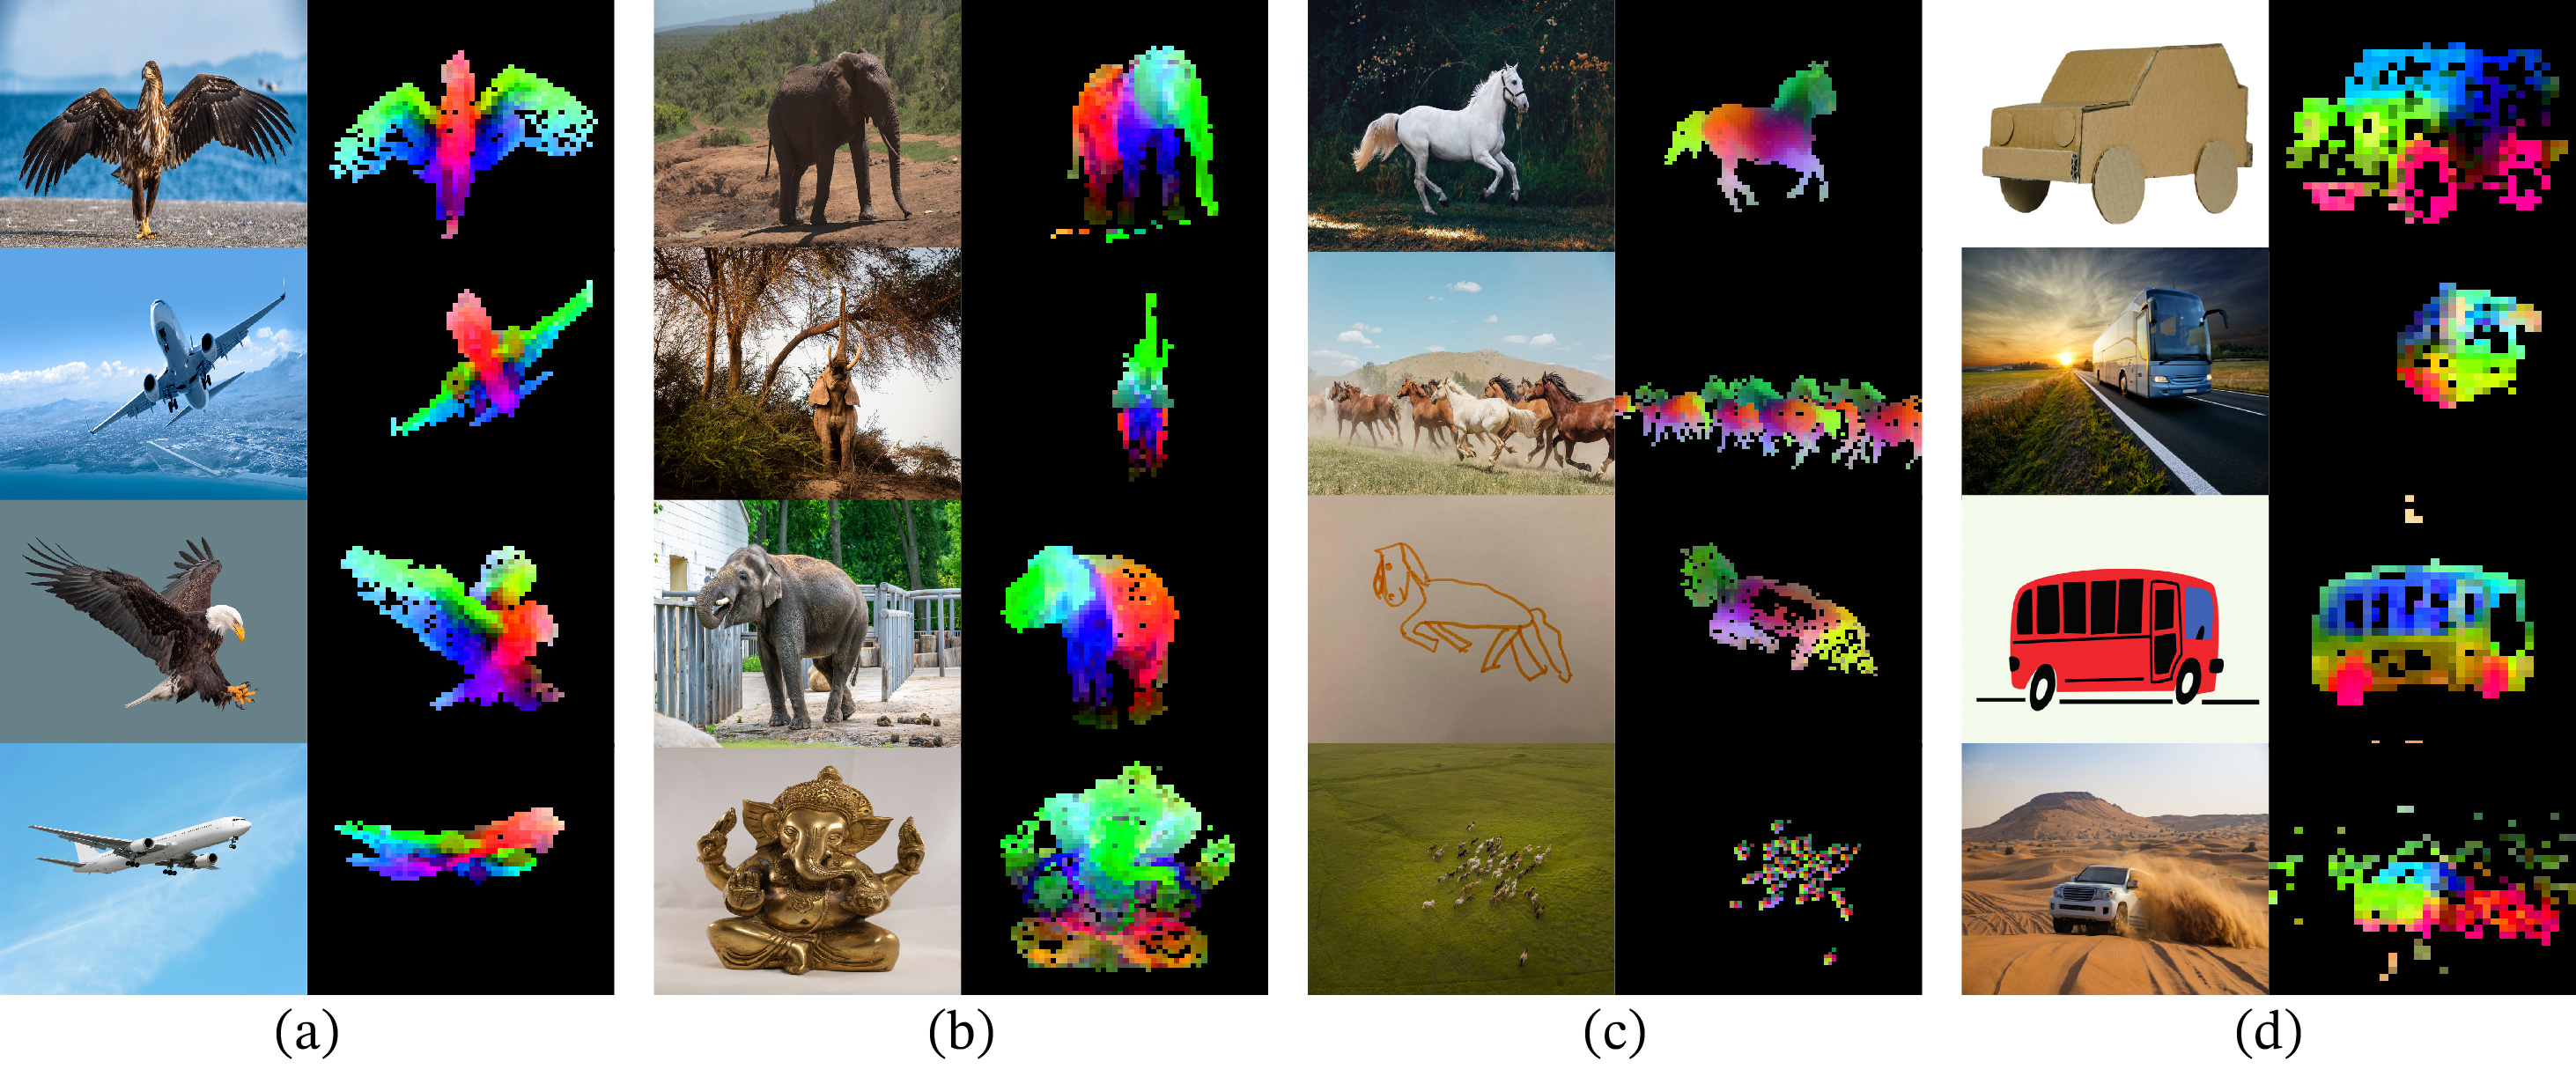
\includegraphics[width=\linewidth]{new-figure-1.jpg}
  \caption{
    \textbf{Visualization of the first PCA components.} We compute a PCA between the patches of the images from the same column (a, b, c and d)   and show their first 3 components.
    Each component is matched to a different color channel. 
    Same parts are matched between related images despite changes of pose, style or even objects.
    Background is removed by thresholding the first PCA component.
  }
  \label{fig:qualitative}
\end{figure*}

An alternative to text-guided pretraining is self-supervised learning ~\citep{caron2018deep, chen2020simple, he2021masked} where features are learned from images alone. 
These approaches are conceptually closer to pretext tasks such as language modeling and can capture information at the image and pixel level~\citep{caron2021emerging}.
Additionally, the features output by self-supervised models have been shown to exhibit various useful properties, and have enabled enabled a wide variety of applications~\citep{amir2021deep, tumanyan2022splicing, ofri2023neural, hamilton2022unsupervised}.
However, despite their potential to learn general-purpose features, most of the advances in self-supervised learning were made in the context of pretraining on a small curated dataset, ImageNet-1k~\citep{russakovsky2015imagenet}.
Some efforts on scaling these approaches beyond ImageNet-1k have been attempted~\citep{caron2019unsupervised, goyal2021self,goyal2022vision}, but they focused on uncurated datasets, which typically lead to a significant drop in the quality of the features.
This is explained by the lack of control over the data quality and diversity, which are essential to produce good features.

In this work, we explore if self-supervised learning has the potential to learn general-purpose visual features if pretrained on a large quantity of curated data.
We revisit existing discriminative self-supervised approaches that learn features at both the image and patch level, such as iBOT~\citep{zhou2021ibot}, and we reconsider some of their design choices under the lens of a larger dataset.
Most of our technical contributions are tailored toward stabilizing and accelerating discriminative self-supervised learning when scaling in model and data sizes.
These improvements make our approach around 2$\times$ faster and require 3$\times$ less memory than similar discriminative self-supervised methods, allowing us to leverage longer training with larger batch sizes. 

Regarding pretraining data, we have built an automatic pipeline to filter and rebalance datasets from an extensive collection of uncurated images.
This pipeline is inspired by pipelines used in NLP~\citep{wenzek2019ccnet}, where data similarities are used instead of external metadata and do not require manual annotation.
A major difficulty when dealing with images in the wild is to rebalance concepts and avoid overfitting on a few dominant modes.
In this work, a naive clustering approach works reasonably well to resolve this issue.
We gathered a small but diverse corpus of 142M images to validate our approach.

Finally, we provide a variety of pretrained visual models, called \OURS, trained with different Vision Transformers~(ViT)~\citep{dosovitskiy2016discriminative} architectures on our data.
We release all the models and the code to retrain \OURS~on any data. 
We validate the quality of \OURS~on various computer vision benchmarks at both image and pixel levels as we scale them, as summarized in Fig.~\ref{tab:pullfig}.
We conclude that self-supervised pretraining alone is a good candidate for learning transferable frozen features that are competitive with the best openly available weakly-supervised models.
